
%\documentclass[twocolumn]{article}
\documentclass[a4paper,10pt]{article}
\title{ Research Statement \\\rq\rq{}Micro-Robotics\rq\rq{}
}
\author{
        Nafiseh Vahabi 
}
%\date{\today}


\usepackage[round]{natbib}
\usepackage[pdftex]{graphicx}
\usepackage{amsmath}
\usepackage{multirow} 
\usepackage {fullpage}
\usepackage[inference,shorthand]{semantic}
\usepackage{fancyvrb}
\usepackage{listings}
\usepackage{comment} 
\usepackage{tikz}
\usepackage[]{caption}
\usepackage{verbatim}


\usetikzlibrary{shadows,arrows,positioning}
% Define the layers to draw the diagram
\pgfdeclarelayer{background}
\pgfdeclarelayer{foreground}
\pgfsetlayers{background,main,foreground}

% Define block styles
\tikzstyle{materia}=[draw, fill=yellow!20, text width=10.0em, text centered,
  minimum height=7.5em,drop shadow]
\tikzstyle{practica} = [materia, text width=12em, minimum width=12em,
  minimum height=3em, rounded corners, drop shadow]
\tikzstyle{texto} = [above, text width=15em, text centered]
\tikzstyle{linepart} = [draw, thick, color=black, -latex', dashed]
\tikzstyle{line} = [draw, thick, color=black, -latex']
\tikzstyle{ur}=[draw, text centered, minimum height=0.01em]
\usetikzlibrary{fadings}
\usetikzlibrary{decorations}
\usepgflibrary{decorations.pathmorphing}

\tikzfading[name=fade out, inner color=transparent!0,
  outer color=transparent!100]

% Define distances for bordering
\newcommand{\blockdist}{1.3}
\newcommand{\edgedist}{1.5}

%\newcommand{\etape}[2]{node (p#1) [etape]
 % {#2}}

\newcommand{\Step}[2]{node (p#1) [practica]
  {\\{ \Large\textit{#2}}}}

% Draw background
\newcommand{\background}[5]{%
  \begin{pgfonlayer}{background}
    % Left-top corner of the background rectangle
    \path (#1.west |- #2.north)+(-1.3,0.01) node (a1) {};
    % Right-bottom corner of the background rectanle
    \path (#3.east |- #4.south)+(+0.3,-0.5) node (a2) {};


    % Draw the background
  % \path[fill=blue!20,rounded corners, draw=black!50, dashed]
     %(-4,-5.2) rectangle (4,1);

   \path[fill=gray!40 ,rounded corners, draw=black, dashed]
     (3.5,-4.2) rectangle (9.55,2.8);

%%%%%%%%%%%%%
% \fill[yellow!10!black] (-1,1) rectangle (6,3);
    %\fill[yellow] (-4,-5.2) rectangle (4,1);
   %\fill[inner color=blue!50!,outer color=blue!10!black] (4.7,-5.2) rectangle (12.5,1);
%%%%%%%%%%%%%%%%%%%%%%%%%%

 \path (a1.east |- a1.south)+(3.5,0.5) node (u1)[texto]
      { \LARGE\textit{ #5}};

      \path (#3.east |- #2.north)+(0,0.25)--(#1.west |- #2.north) node[midway] (#5-n) {};
      \path (#3.east |- #2.south)+(0,-0.35)--(#1.west |- #2.south) node[midway] (#5-s) {};
      \path (#3.east |- #2.north)+(0.7,0)--(#3.east |- #4.south) node[midway] (#5-w) {};
  \end{pgfonlayer}}

\newcommand{\transreceptor}[3]{%
  \path [linepart] (#1.east) -- node [center]
    {\large #2} (#3);}

%---------------------------------------------------- Start the document----------------------------------------------

\begin{document}


\maketitle


\section{Research Background}







\section{Objective and methodology}

\begin{figure}
\centering
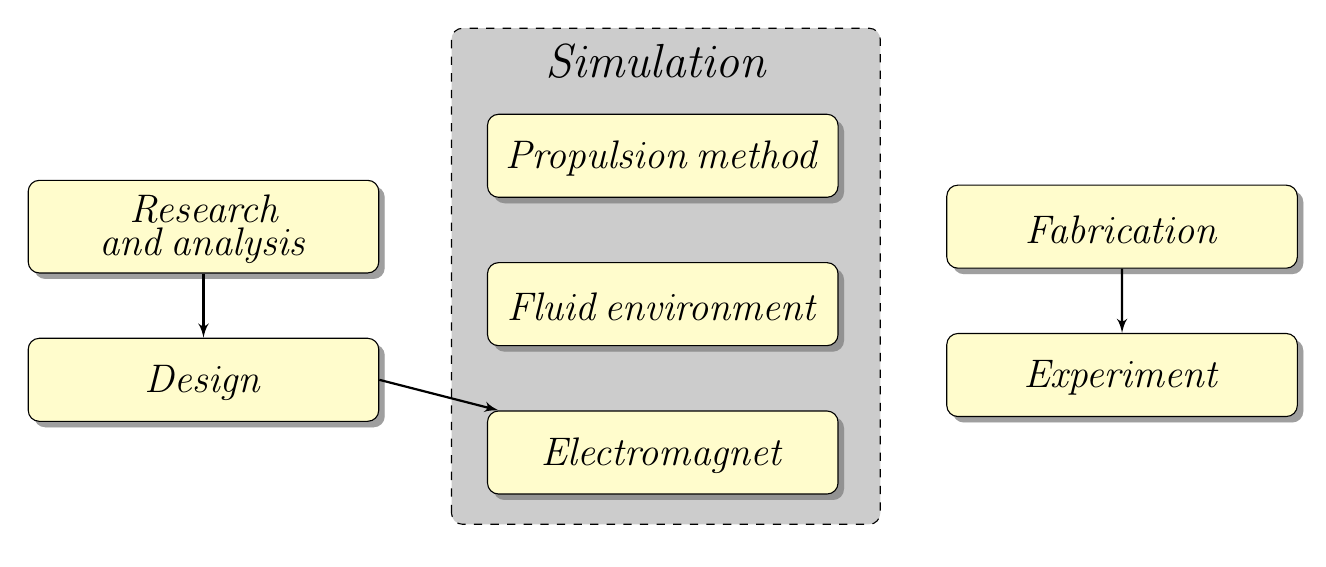
\begin{tikzpicture}[scale=0.90,[every node/.style={font=\large,
  minimum height=0.5cm,minimum width=0.5cm},]]

  % Draw diagram elements
  \path \Step{1}{Research and analysis};
  \path (p1.south)+(0.0,-1.5) \Step{2}{Design};

  \path (p1.east)+(4.0,1.0) \Step{3}{Propulsion method};
   \path (p3.south)+(0.0,-1.5) \Step{4}{Fluid environment};
   \path (p4.south)+(0.0,-1.5) \Step{5}{Electromagnet};


  \path (p3.east)+(4.0,-1.0) \Step{6}{Fabrication};
    \path (p6.south)+(0.0,-1.5) \Step{7}{Experiment};

 % \path (p3.south)+(4.10,-2.0) \Step{7}{Integrating e-AR and robot};
 % \path (p9.south)+(0.0,-1.5) \Step{10}{Laparoscopy Robot};


  % Draw arrows between elements
  \path [line] (p1.south) -- node [above] {} (p2);
 \path [line] (p2.east) -- node [above] {} (p5);
  %\path [line] (p1.east) -- node [above] {} (p4);

  %\path [line] (p2.east) -- node [above] {} (p5);
  %\path [line] (p3.east) -- node [above] {} (p6);
% \path [line] (p6.south) -- node [above] {} (p7);

  %\path [line] (p4.south) -- node [above] {} (p5);
  %\path [line] (p3.south) -- node [above] {} (p7);
  \path [line] (p6.south) -- node [above] {} (p7);



   \background{p3}{p3}{p5}{p5}{Simulation }



%%%%%%%%%%%%%% CHANGED%%%%%%%%%%%%%
\end{tikzpicture}									   %
\caption{The proposed system architecture. The stages are required %
to develope a swimming magnet microrobot.}						   
\label{Architec}										   %
\end{figure}										   %	
												   %
%%%%%%%%%%%%%% CHANGED%%%%%%%%%%%%%



\section{Suitability}  



\nocite{balcanefficient}


%{abbrvnat}
\bibliographystyle{abbrvnat}
\bibliography{reference}


\end{document}
This is never printed
